\begin{frame}{Metode bagi-dua (\textit{bisection})}

Metode bagi-dua bekerja dengan input tebakan awal $x_l$ dan $x_u$,
(dengan $x_l$ < $x_u$) yang
mengapit akar, artinya akar berada diantara $x_l$ dan $x_u$.
Jika $f(x)$ bernilai real dan kontinu dan
$$
f(x_l) f(x_u) < 0
$$
atau jika $f(x_l)$ dan $f(x_u)$ berbeda tanda maka ada
akar diantara $x_l$ dan $x_u$.
Untuk metode bagi-dua, tebakan akar diberikan oleh titik tengah
dari $x_l$ dan $x_u$:
$$
x_{r} = \frac{x_l + x_u}{2}
$$
Pada iterasi selanjutnya, salah satu dari $x_l$ dan $x_u$ akan
digantikan dengan $x_r$, bergantung dari tanda dari $f(x_r)$.

\end{frame}


\begin{frame}{Metode bagi-dua (\textit{bisection})}
Langkah-langkah metode bagi-dua:
\begin{itemize}\tightlist
\item STEP 1: Pilih $x_l$ dan $x_u$ yang memenuhi $f(x_l) f(x_u) < 0$
\item STEP 2: Hitung estimasi akar:
  \begin{equation*}
  x_r = \frac{x_l + x_u}{2}
  \end{equation*} 
\item STEP 3: Perbarui selang $[x_l, x_u]$:
  \begin{itemize}
  \item Jika $f(x_l) f(x_r) < 0$, ganti atau perbarui nilai $x_u \leftarrow x_r$
    kemudian kembali ke STEP 2.
  \item Jika $f(x_l) f(x_r) > 0$, ganti atau perbarui nilai $x_l \leftarrow x_r$
    kemudian kembali ke STEP 2.
  \item Jika $f(x_l) f(x_r) = 0$ atau nilai absolut dari $f(x_r)$ sudah lebih kecil
    dari nilai toleransi tertentu maka hentikan perhitungan.
  \end{itemize}
\end{itemize}

\end{frame}


\begin{frame}{Metode bagi-dua (\textit{bisection})}

{\centering
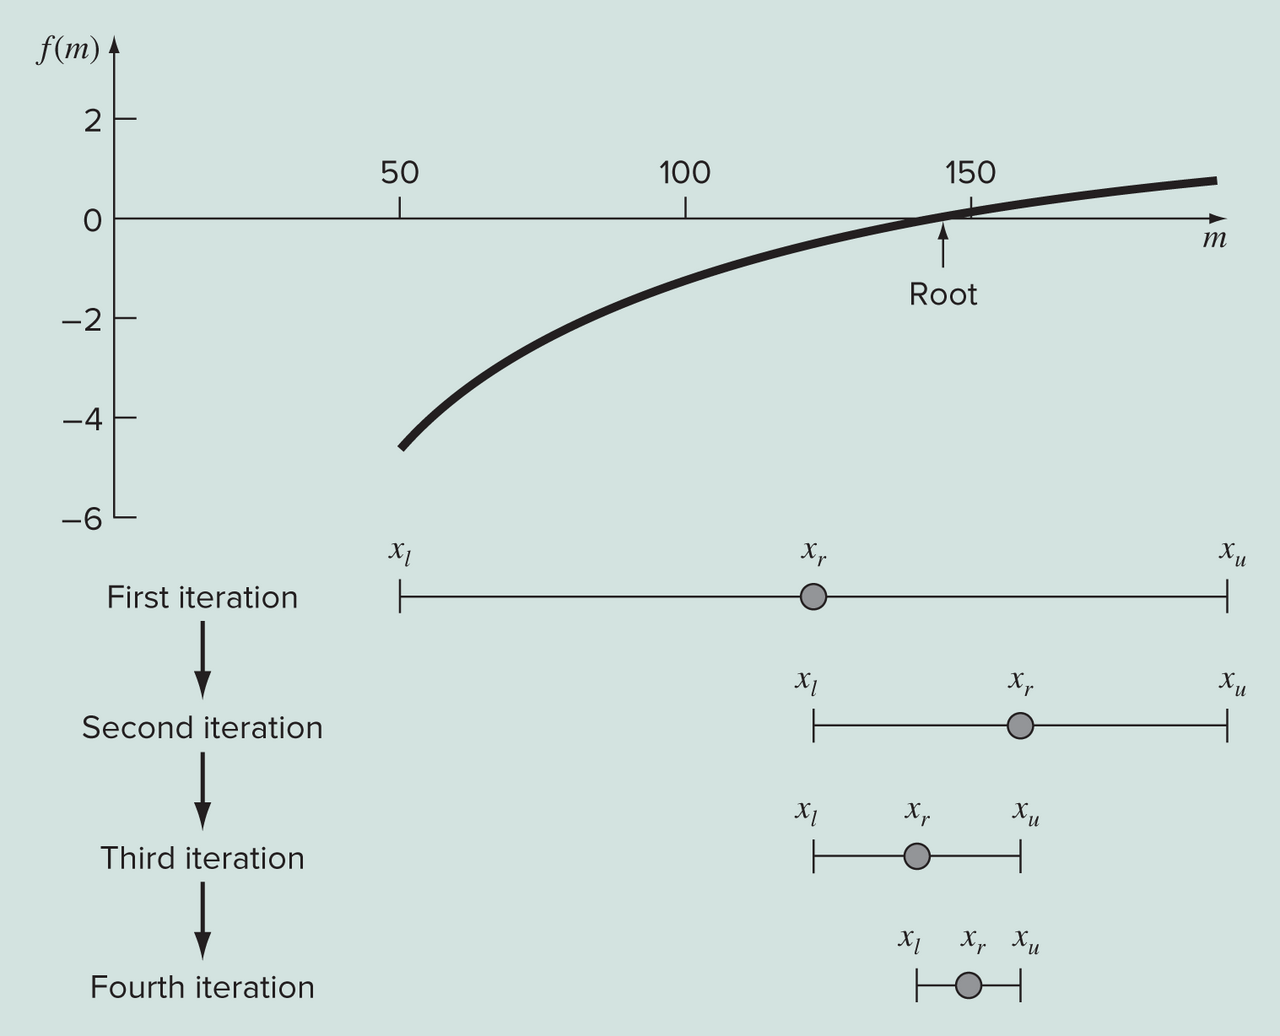
\includegraphics[height=0.8\textheight]{../chapra_python/Chapra_Fig_5_5.png}
\par}

\end{frame}


\begin{frame}{Contoh metode bagi-dua}

Contoh proses iterasi untuk $f(c)$ dengan tebakan selang $[12,16]$:

{\centering
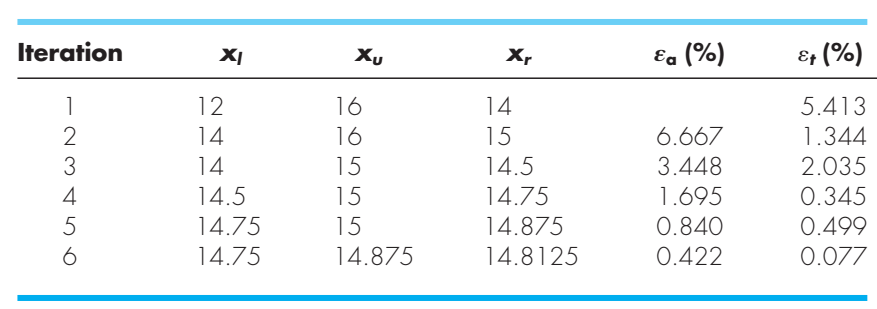
\includegraphics[height=0.5\textheight]{../chapra_7th/Chapra_Table_Example_5_4.png}
\par}

\end{frame}


\begin{frame}{Metode \textit{regula-falsi}}
\fontsize{9}{10}\selectfont

\begin{columns}
  
  \begin{column}{0.5\textwidth}
  Ide dari metode regula-falsi mirip dengan metode bagi-dua. Perbedaannya
  adalah estimasi akar diperoleh dari perpotongan garis lurus yang menghubungkan
  antara $f(x_l)$ dan $f(x_u)$ dengan sumbu-$x$.

  Dari gambar:
  $$
  \frac{f(x_l)}{x_r - x_l} = \frac{f(x_u)}{x_r - x_u}
  $$
  sehingga diperoleh:
  $$
  x_r = \frac{x_u f(x_l) - x_l f(x_u)}{f(x_l) - f(x_u)}
  $$
  atau (alternatif):
  $$
  x_r = x_u - \frac{f(x_u)(x_l - x_u)}{f(x_l) - f(x_u)}
  $$
  \end{column}

  \begin{column}{0.5\textwidth}
  {\centering
  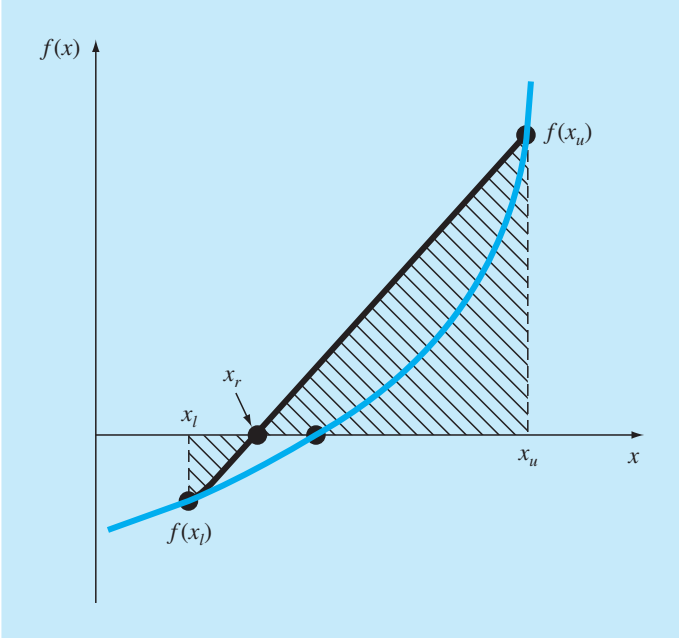
\includegraphics[height=0.7\textheight]{../chapra_7th/Chapra_Fig_5_12.png}
  \par}
  \end{column}

\end{columns}

\end{frame}


\begin{frame}{Metode \textit{regula-falsi}}
\fontsize{10}{11}\selectfont

\begin{columns}

  \begin{column}{0.5\textwidth}
  Implementasi metode \textit{regula-falsi} mirip dengan metode bagi-dua.
  Perbedaannya hanya pada persamaan yang digunakan untuk $x_r$.

  Biasanya metode \textit{regula-falsi} membutuhkan iterasi yang lebih sedikit
  untuk konvergen ke akar dibandingkan dengan metode bagi-dua, meskipun pada kasus
  tertentu metode bagi-dua dapat lebih cepat konvergen. Pada kasus ini, kita bisa
  mengatasinya dengan cara menggunakan metode bagi-dua jika konvergensi metode
  \textit{regula-falsi} stagnan setelah beberapa iterasi (Lihat Contoh 5.6 pada Chapra
  dan metode \textit{regula-falsi} yang dimodifikasi).
  \end{column}

  \begin{column}{0.5\textwidth}
  {\centering
  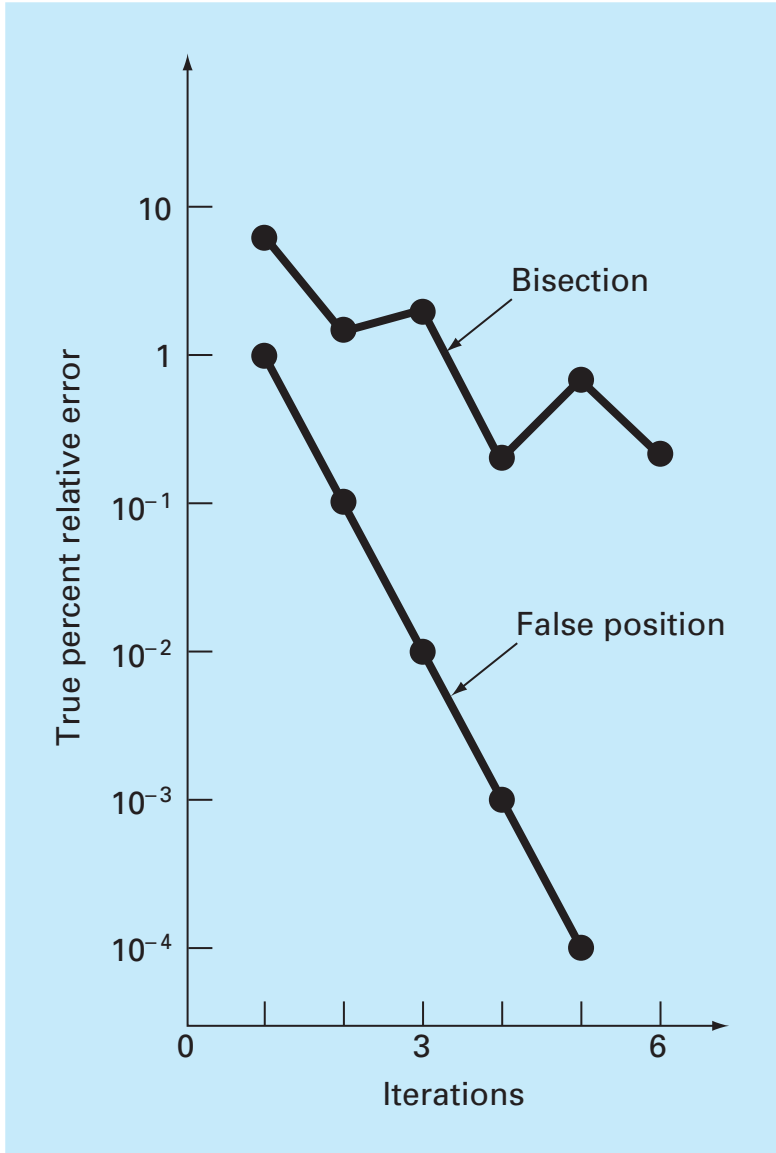
\includegraphics[height=0.8\textheight]{../chapra_7th/Chapra_Fig_5_13.png}
  \par}
  \end{column}

\end{columns}

\end{frame}